\documentclass[aps,superscriptaddress,twocolumn,nopreprintnumbers,floatfix,groupedaddress]{revtex4-1}
\usepackage{amssymb}
\usepackage{amsmath}
\usepackage{graphicx}
\usepackage{dcolumn}
\usepackage{hyperref}
\usepackage{color,units}
\usepackage{lineno}
\usepackage{xspace}
\usepackage{mathtools}
\usepackage{physics}
\usepackage{acronym}


\newcommand{\bilby}{{\sc Bilby}\xspace}
\newcommand{\lal}{{\sc LAL}\xspace}
\newcommand{\lalsuite}{{\sc LALSuite}\xspace}
\newcommand{\lalsimulation}{{\sc LALSimulation}\xspace}
\newcommand{\sur}{{\sc NRHybSur3dq8}\xspace}
\newcommand{\Z}{\mathcal{Z}}
\newcommand{\M}{\mathcal{M}}
\renewcommand{\L}{\mathcal{L}}
\newcommand{\BF}{\mathcal{BF}}
\newcommand{\proposal}{proposal}
\newcommand{\target}{target}
\newcommand{\ep}[1]{\textcolor{red}{[EP: #1]}}
\newcommand{\et}[1]{\textcolor{blue}{[ET: #1]}}
\newcommand{\ct}[1]{\textcolor{green}{[CT: #1]}}

\newcommand{\nessai}{{\sc Nessai}\xspace}
\newcommand{\vitamin}{{\sc VItamin}\xspace}
\newcommand{\bilbypipe}{{\sc bilby\_pipe}\xspace}
\newcommand{\lalinference}{{\sc LALInference}\xspace}
\newcommand{\dynesty}{{\sc dynesty}\xspace}
\newcommand{\cpnest}{{\sc cpnest}\xspace}
\newcommand{\nflows}{{\sc nflows}\xspace}
\newcommand{\pytorch}{{\sc PyTorch}\xspace}
\newcommand{\corner}{{\sc corner}\xspace}
\newcommand{\matplotlib}{{\sc matplotlib}\xspace}
\newcommand{\seaborn}{{\sc seaborn}\xspace}
\newcommand{\numpy}{{\sc NumPy}\xspace}
\newcommand{\scipy}{{\sc SciPy}\xspace}
\newcommand{\pandas}{{\sc pandas}\xspace}
\newcommand{\python}{{\sc Python}\xspace}
\newcommand{\imrphenomp}{{\sc IMRPhenomPv2}\xspace}


\newcommand{\figwidth}{8.6cm}
\newcommand{\onehalffigwidth}{12.9cm}
\newcommand{\doublefigwidth}{17.2cm}

\begin{document}

\title{Explainable Deep-learning: Monte Carlo methods for Gravitational-Wave Inference}

\author{2259886}
%\email{ethan.payne@ligo.org}
\affiliation{%
	SUPA, School of Physics and Astronomy \\
	University of Glasgow \\
	Glasgow G12 8QQ, United Kingdom
}%

\date{\today}

\begin{abstract}
My 250 word abstract goes here...
\end{abstract}

\maketitle

\acrodef{GW}[GW]{Gravitational wave}
\acrodef{BBH}[BBH]{binary black hole}
\acrodef{EM}[EM]{electromagnetic}
\acrodef{CBC}[CBC]{compact binary coalescence}
\acrodef{BNS}[BNS]{binary neutron star}
\acrodef{NSBH}[NSBH]{neutron star black hole}
\acrodef{PSD}[PSD]{power spectral density}
\acrodef{ELBO}[ELBO]{evidence lower bound}
\acrodef{LIGO}[LIGO]{advanced Laser Interferometer Gravitational wave Observatory}
\acrodef{CVAE}[CVAE]{conditional variational autoencoder}
\acrodef{KL}[KL]{Kullback--Leibler}
\acrodef{GPU}[GPU]{graphics processing unit}
\acrodef{LVC}[LVC]{LIGO-Virgo Collaboration}
\acrodef{PP}[p-p]{probability-probability}
\acrodef{SNR}[SNR]{signal-to-noise ratio}

\section{Introduction}\label{intro}

\textbf{\textcolor{red}{Figs: LIGO Cumulative events}}

\textbf{\textcolor{red}{Figs: Hunter's Vit Schematic}}



Remember to signpost rest of paper at end of this section!

%\subsection{}
%
\subsection{\vitamin: User-Friendly Inference}\label{vit}
%
%\subsection{Structure}
%
%\subsection{Training}
%
%\subsection{Results}

\section{Theoretical Framework}\label{theory}

Need to mention metropolis hastings it seems!

Don't apply it to our sitaution at this stage, just straight theory and equations (Section \ref{methods} deals with taking these eqns arnd applying them to our situation)

\subsection{Monte Carlo Framework}\label{theory:monte}

\subsection{SIR Framework}\label{theory:sir}

Do theory on normal IS and then say that SIR is an monte carlo approach/approx to normal IS then give equations for bot (talk about the NEW IMPROVED SIR method (link to Section \ref{future}))

%
%\subsection{Theoretical Framework}\label{monte:theory}

\section{Methodology}\label{methods}

Apply the intro/theory mateiral to our case, JUSTIFY scientific decisions like number of samples, batch size, npars!!

\subsection{Model Training}

\begin{figure}
	\centering
	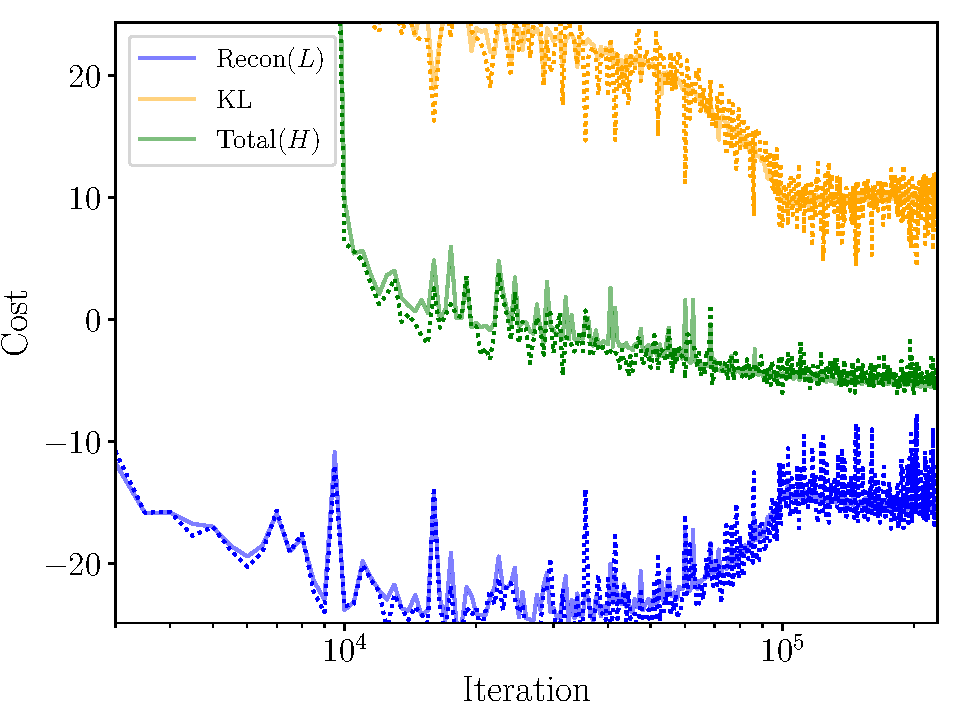
\includegraphics[width=\figwidth]{figs/cost.pdf}
	\caption{Example of how a normalising flow trained on a set of live points can produce samples within current iso-likelihood contour for simple two-dimensional parameter space. \textbf{Top:} example of training samples in the physical space $\physical$ and learned mapping to the latent space $\latent$ with the iso-likelihood contour for the current \textit{worst point} shown in orange. \textbf{Middle:} samples drawn from a truncated Guassian within the iso-likelihood contour in $\latent$ and mapped to $\physical$ using the inverse mapping. \textbf{Bottom:} pool of accepted samples after applying rejection sampling until 1000 points are obtained shown in both $\latent$ and $\physical$.}
	\label{fig:learning_contours}
\end{figure}

\textbf{\textcolor{red}{Figs: loss plot}}

\textbf{\textcolor{red}{Tables: training hypers in table}}

\textbf{\textcolor{red}{Figs: initial corner plot? (to talk about params and how posteriors aren't perfect)}}

Need this cornerplot here to talk about how it doesn't `get' the multimodal dists, which after resampling it does!

\subsection{Likelihood Estimates}

\textbf{\textcolor{red}{Figs: Monte flowchart}}

\subsection{Importance Resampling}


\section{Results}\label{results}

\subsection{Self-consistency}

\textbf{\textcolor{red}{Figs: Self consist corner plot}}

\subsection{Reproducibility}

Talk about how 'binning' is preventing proper error profile acorss the likelihood range, (not present in the \dynesty case)

\textbf{\textcolor{red}{Figs: z batch vs sigma}}

\textbf{\textcolor{red}{Figs: sigma gaussians for different z batch}}

\textbf{\textcolor{red}{Figs: scatter vit vit}}

\textbf{\textcolor{red}{Figs: scatter vit dynesty}}

\subsection{Importance Resampling}


\textbf{\textcolor{red}{Figs: Final corner plot (big)}}


\section{Future Work}\label{future}

As we find ourself in a proof-of-concept mode, there is justification of a section dedicated to the next steps leading towards production of this code.

\section{Conclusions}\label{conc}

This is section has to encapsulate everything we did so that after the abstract a reader can go here and see if they want to buy the paper or not!

\section{Acknowledgements}

Thanks to Chris and Hunter and Michael and Daniel.

Paragraph on the software used \bilby\cite{bilby} 
%\clearpage
\bibliography{refs}




\end{document}